\chapter{Experimental Protocol}\label{Chapter:5}

In this chapter the design aspects introduced in previous chapters (\ref{ch:2},\ref{ch:3},\ref{Chapter:4}) are brought together and find their practical application. The goal is to produce measurable performance results by applying of preprocessing and machine learning algorithms.

The general pattern that this chapter follows is partially attributed to the CRISP-DM process (see Figure~\ref{fig:crisp-dm}) and contains three sub-processes: \textit{DataPreparation, Modelling, Evaluation}. Each of them contains techniques previously described in this thesis. 

\begin{figure}[h!]
    \centering
    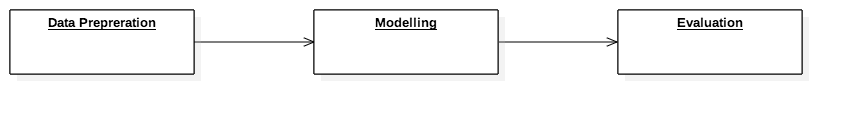
\includegraphics[scale=0.5]{Graphics/DeploymentDiagram1.png}
    \caption{A general experiment pattern.} %footnote?
    \label{fig:dep-dia}
\end{figure}

An experiment is defined as an process that follows the general experimental pattern (see Figure~\ref{fig:dep-dia}), where the particular methods (see Tables~\ref{tab:data-pred-methods}, \ref{tab:machine-learn-tech}, \ref{tab:res-ev}) and their parameters can vary.

\section{Experimental Setting} \label{ch:5:ES}

\subsection{Dataset Description}

The initial data set has \(95.951\) instances with \(1.804\) features per instance. Each instance represents a single credit-application (a detailed overview of underlying data can be found in Chapter~\ref{Ch:2:FeatureDesc}). 

The data is divided into \textit{Training/Validation/Test} sets in the proportion\footnote{A common suggested size for the training set is $60\%-80\%$~\cite{UBHD65918158}.} \((\approx60\%/\approx30\%/\approx10\%)\). All instances that are labeled as \textit{Fraud}~\((743)\) are assigned to the test set since the predictive algorithms expects \textit{Positive} and \textit{Unlabeled} data only. Thus, fraud instances are not a part of training/validation sets.

\begin{table}[ht!]
\centering
 \begin{tabular}{|l|l|}\hline
  Operation&Reference\\ \hline
 Removing Corrupted Instances  & \ref{Ch:2:RCD} \\ \hline
        Categorical to Numeric Transformation & \ref{Ch:2:CTNT} \\
     \hline 
      Missing Value Imputation & \ref{Ch:2:MVI} \\
     \hline 
     Removing Zero- and Near-Zero Variance Features  & \ref{Ch:2:RNZVF} \\
     \hline 
     Principle Component Analysis (PCA) & \ref{Ch:2:PCA} \\
     \hline 
        \end{tabular}
\caption{Operations included into data preprocessing.}
\label{tab:data-pred-methods} 
\end{table}

\begin{table}[ht!]
\centering
 \begin{tabular}{|l|l|}\hline
         Method & Reference\\
        \hline
        Two-Class SVM & \ref{Chapter:SVM} \\
        \hline
        One-Class SVM & \ref{Chapter:OC-SVM} \\
        \hline
        PUL &  \ref{Chapter:PUL} \\
        \hline
        PUL Ensemble &  \ref{Chapter:Ensemble} \\
        \hline
    \end{tabular}
 \caption{Machine learning methods used in experiments.}
\label{tab:machine-learn-tech} 
\end{table}

\begin{table}[ht!]
    \centering
        \begin{tabular}{|c|c|}
        \hline
        Technique&Reference\\
        \hline
        ROC analysis & \ref{Chapter:4:ROC} \\
        \hline
        \end{tabular}
        \caption{Performance evaluation techniques used in experiments.}
    \label{tab:res-ev}
\end{table}



\subsection{Preprocessing Settings}\label{ch:prepro:setting}

Below the configuration settings for (all) the preprocessing operations (see Table~\ref{tab:data-pred-methods}) used in the experiment are given:

\begin{itemize}
    \item Corrupted instances will be completely excluded from the data set.
    
    \item The imputation of missing values is done by imputing the \textit{median} value for numerical features and by adding of a \textit{new level}, such as 'OTHER', to the categorical features.
    
    \item All categorical features are then transformed to a numerical representation.
    
    \item \textit{Low variance} features are removed with thresholds \(freqCut = 95/5\) (the cutoff for the ratio of the most common value to the second most common value) and \(uniqueCut = 10\) (the cutoff for the percentage of distinct values out of the total number of instances). 
    
    \item Data dimensionality is reduced with the \textit{PCA} analysis in order to preserve \(\approx95\%\) of the total data variance. The R implementation of PCA explicitly performs the zero-mean, unit-variance normalization (scaling) of each feature.
    
\end{itemize}

All machine learning methods are trained \textbf{with} and \textbf{without} PCA. Since the PCA analysis is configured to capture \(95\%\) of the total variance in data (see the configuration in section~\ref{ch:prepro:setting}), the impact of the other \(5\%\) on the prediction model is an interesting case to observe.

To outline the impact of the data preprocessing - an additional experiment is performed. It includes the training of the \textit{one-class SVM} on the data when all but the categorical-to-numeric conversion was omitted.

\subsection{Modelling Settings}\label{ch:modelling-settings}

There are three different models (one-class SVM, PUL and PUL Ensemble; two-class SVM is a part of the last two models).

All classification tasks use the \textit{stratified ten-fold cross-validation} carried out on the training data to find the optimal values of model parameters. The training data is randomly divided into \(k\) chunks (folds) while preserving the original class ratio in each chunk as much as possible. A classifier is then trained \(k\) times: One chunk is used for the validation and the remaining \(k-1\) are used for  training~\cite{Kohavi95}.

For SVMs regardless of their type, the Radial Basis Function (RBF) kernel was chosen, which implies two parameters: \(\sigma\) - kernel width and \(C\) - penalty cost.

As our data is class-imbalanced (see in Chapter~\ref{Ch:2:SSummary} the Table~\ref{tab:instance-summary} for the label distribution), the class-weighted version of the SVM was used, which an extra parameter - class weight.

During the cross-validation, the optimal value of the kernel width was first determined prior to the start of cross-validation. After that, the optimal values of the penalty cost and the class weight are determined by going through every possible combination of these two parameters. The possible values for the penalty cost are ($0.25,0.5,1.0,2.0$), whereas the possible values for the class weight are ($1.0,2.0,3.0,4.0$). Thus, there are $16$ combinations to test\footnote{The possible values are automatically provided by the R library \textit{Caret}~\cite{JSSv028i05}, used to compute the models in this Thesis.}. A small number of combinations is caused by the high computational cost of the cross-validation and SVM training.

When creating a PUL ensemble, 10 PUL classifiers were used, each trained on \(11.514\) positive and \(5.757\) unlabeled instances, sampled from the original dataset.

Two types of voting are used for combining predictions of individual classifiers:

\begin{itemize}
    \item A \textit{majority voting}, where the class of the majority determines the final class.
    \item A \textit{custom voting}, where at least \textbf{three} votes are required to classify an instance as fraudulent.
\end{itemize}

\section{Experimental Results}\label{Chapter:5:Results}

\subsection{Preprocessing Results}
The effect of preprocessing on the number of features and the number of instances is analyzed below.

\paragraph*{Impact on Features} \hfill \break
Figure~\ref{fig:features-preprocessing} shows the change in the number of features after each preprocessing operation. The preprocessing reduced the number of features from \(1.804\) to \(271\), this corresponds reduction by \(\approx85\%\). 

\begin{figure}[h!]
    \centering
    \fbox{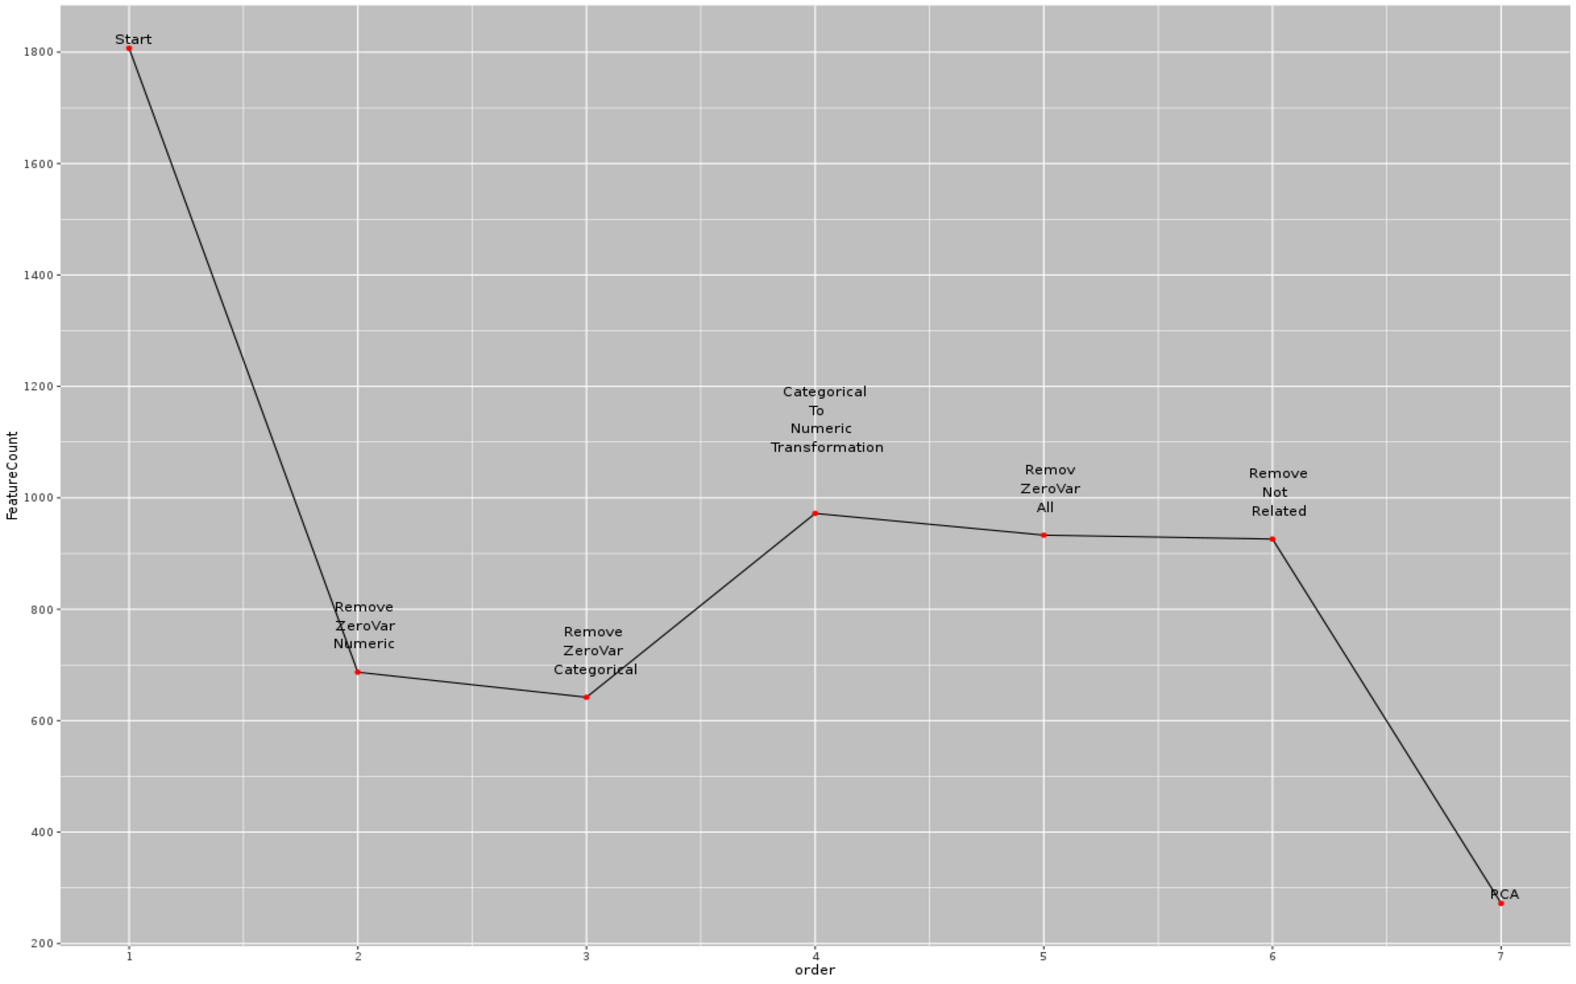
\includegraphics[scale=0.25]{Graphics/preprocessing-features.png}}
    \caption{Changes in the feature amount during the preprocessing.}
    \label{fig:features-preprocessing}
\end{figure}

Table~\ref{tab:feature-reduction} present a detailed description of preprocessing operations visualized at Figure~\ref{fig:features-preprocessing} and their impact on the amount of features after the particular operation was applied.
\begin{table}[h!]
  \begin{center} 
    \caption{The preprocessing impact on the amount of Features.}
    \label{tab:feature-reduction}
   \hspace*{-1cm} \begin{tabular}{|l|c|c|}\hline
    \textit{Number} & \textit{Operation} & \textit{Features left} \\
      \hline
     (1.) & Start & \(1.807\) \\ 
     \hline
     (2.) & Removing Zero- and Near-Zero Variance from Numerical Features  &  \(687\) \\
     \hline
     (3.) & Removing Zero- and Near-Zero Variance from Categorical Features &  \(642\) \\
     \hline
     (4.) & Categorical To Numeric Transformation &  \(972\) \\
     \hline
     (5.) &  Removing Zero- and Near-Zero Variance from all existing Features &  \(933\) \\
     \hline
     (6.) &  Removing Features not necessary for the further training process (e.g \textit{Label}, \textit{ID}...) &  \(926\) \\
     \hline
     (7.) & Principal Component Analysis (capture \(95\%\) of the avaliable variance) &  \(272\) \\
     \hline
    \end{tabular}
  \end{center}
\end{table}

\paragraph*{Impact on Instances and their Values} \hfill \break
Removing of instances contaminated by data acquisition errors reduced the sample size by \(\approx1\%\) to \(95.829\) instances. There were a lot of missing values in the data: $\approx40\%$ of all numeric values and about $\approx53\%$ of all categorical and logical values were imputed.

\subsection{Modelling / Machine Learning Results}
The test set comprises \(2229\) instances. As SVMs do not naturally return probabilities as an output, the confusion matrices are reported instead.

\paragraph*{One-Class SVM} \hfill \break
The test results are shown below (see Figure~\ref{tables:confusion-matrices-oneclass}). The positive impact of preprocessing is clearly seen as without it results are greatly inferior to those with it. However, it is hard to judge on the effect of PCA: with PCA the number of detected fraud cases is almost twice higher than when PCA is not performed; however, this is done at the expense of the correctly predicted positive cases.
\begin{figure}[ht!]
\begin{multicols}{3}
\hspace*{-2cm}
\begin{tikzpicture}[
box/.style={draw,rectangle,minimum size=1cm,text width=0.75cm,align=left}]
\matrix (conmat) [row sep=.1cm,column sep=.1cm] {
\node (tpos) [box,
    label=left:\( \mathbf{P} \),
    label=above:\( \mathbf{P} \),
    ] {\textcolor{green}{\(751\)}};
&

\node (fneg) [box,
    label=above right:\textcolor{green}{\textbf{756}},
    label=above:\textbf{N}] {\textcolor{red}{\(738\)}};
\\
\node (fpos) [box,
    label=below left:\textbf{2229},
    label=left:\( \mathbf{N} \)] {\textcolor{red}{\(735\)}};
&
\node (tneg) [box] {\textcolor{green}{\(5\)}};
\\
};
\node [left=.05cm of conmat,text width=1.5cm,align=right] {\textbf{predicted}};
\node[above=1.5cm of conmat]{\textbf{One Class SVM} };
\node[above=0.9cm of conmat]{\textcolor{blue}{\textit{no preprocessing}} };
\node [above=.05cm of conmat] {\textbf{actual value}};
\end{tikzpicture}

\begin{tikzpicture}[
box/.style={draw,rectangle,minimum size=1cm,text width=0.75cm,align=left}]
\matrix (conmat) [row sep=.1cm,column sep=.1cm] {
\node (tpos) [box,
    label=left:\( \mathbf{P} \),
    label=above:\( \mathbf{P} \),
    ] {\textcolor{green}{\(537\)}};
&
\node (fneg) [box,
    label=above:\textbf{N},
    label=above right:\textcolor{green}{\textbf{977}},
    ] {\textcolor{red}{\(303\)}};
\\
\node (fpos) [box,
    label=left:\( \mathbf{N} \),
    label=below left:\textbf{2229}
    ] {\textcolor{red}{\(949\)}};
&
\node (tneg) [box,
    ] {\textcolor{green}{\(440\)}};
\\
};
\node[above=1.5cm of conmat]{\textbf{One Class SVM} };
\node[above=0.9cm of conmat]{\textcolor{blue}{\textit{PCA}}};
\node [above=.05cm of conmat] {\textbf{actual value}};
\end{tikzpicture}

\begin{tikzpicture}[
box/.style={draw,rectangle,minimum size=1cm,text width=0.75cm,align=left}]
\matrix (conmat) [row sep=.1cm,column sep=.1cm] {
\node (tpos) [box,
    label=left:\( \mathbf{P} \),
    label=above:\( \mathbf{P} \),
    ] {\textcolor{green}{\(1157\)}};
&
\node (fneg) [box,
    label=above:\textbf{N},
    label=above right:\textcolor{green}{\textbf{1383}},
    ] {\textcolor{red}{\(517\)}};
\\
\node (fpos) [box,
    label=left:\( \mathbf{N} \),
    label=below left:\textbf{2229}
    ] {\textcolor{red}{\(329\)}};
&
\node (tneg) [box,
    ] {\textcolor{green}{\(226\)}};
\\
};
\node[above=1.5cm of conmat]{\textbf{One Class SVM}};
\node[above=0.9cm of conmat]{\textcolor{blue}{\textit{no PCA} }}; 
\node [above=.05cm of conmat] {\textbf{actual value}};
\end{tikzpicture}
\end{multicols}
    \caption{Confusion Matrices visualizing the Performance of the one-class SVM.}
    \label{tables:confusion-matrices-oneclass}
\end{figure}


\paragraph*{PUL} \hfill \break
In the case of PUL, PCA harmed performance as can be seen in Figure~\ref{tables:confusion-matrices-pul} for both positive and negative cases. The number of correctly predicted fraud cases was significantly higher without PCA. 

\begin{figure}[ht!]
\begin{multicols}{2}
%\hspace*{-1cm}
\begin{tikzpicture}[
box/.style={draw,rectangle,minimum size=1cm,text width=0.75cm,align=left}]
\matrix (conmat) [row sep=.1cm,column sep=.1cm] {
\node (tpos) [box,
    label=left:\( \mathbf{P} \),
    label=above:\( \mathbf{P} \),
    ] {\textcolor{green}{\(1389\)}};
&
\node (fneg) [box,
    label=above:\textbf{N},
    label=above right:\textcolor{green}{\textbf{1555}},
    ] {\textcolor{red}{\(577\)}};
\\
\node (fpos) [box,
    label=left:\( \mathbf{N} \),
    label=below left:\textbf{2229}
    ] {\textcolor{red}{\(97\)}};
&
\node (tneg) [box,
    ,
    ] {\textcolor{green}{\(166\)}};
\\
};
\node [left=.05cm of conmat,text width=1.5cm,align=right] {\textbf{predicted}};
\node[above=1.5cm of conmat]{\textbf{PUL}};
\node[above=0.9cm of conmat]{\textcolor{blue}{\textit{PCA}}};
\node [above=.05cm of conmat] {\textbf{actual value}};
\end{tikzpicture}

\begin{tikzpicture}[
box/.style={draw,rectangle,minimum size=1cm,text width=0.75cm,align=right}]
\matrix (conmat) [row sep=.1cm,column sep=.1cm] {
\node (tpos) [box,
    label=left:\( \mathbf{P} \),
    label=above:\( \mathbf{P} \),
    ] {\textcolor{green}{\(1397\)}};
&
\node (fneg) [box,
    label=above:\textbf{N},
    label=above right:\textcolor{green}{\textbf{1637}},
    ] {\textcolor{red}{\(503\)}};
\\
\node (fpos) [box,
    label=left:\( \mathbf{N} \),
    label=below left:\textbf{2229}
    ] {\textcolor{red}{\(89\)}};
&
\node (tneg) [box,
    ,
    ] {\textcolor{green}{\(240\)}};
\\
};
\node [above=1.5cm of conmat] {\textbf{PUL}};
\node[above=0.9cm of conmat]{\textcolor{blue}{\textit{no PCA} }}; 
\node [above=.05cm of conmat] {\textbf{actual value}};
\end{tikzpicture}
\end{multicols}
\caption{Confusion Matrices visualizing the Performance of the PUL.}
    \label{tables:confusion-matrices-pul}
\end{figure}

\paragraph*{PUL Ensemble} \hfill \break
The detailed results among ensembles are provided in Figure~\ref{tables:confusion-matrices-ensemble}, the highest accuracy was achieved by the ensemble without PCA preprocessing and with custom voting (custom voting is been introduced in section~\ref{ch:modelling-settings}) - This is the highest accuracy in this thesis!
\begin{figure}[ht!]
\begin{multicols}{3}
\hspace*{-2cm}
\begin{tikzpicture}[
box/.style={draw,rectangle,minimum size=1cm,text width=0.75cm,align=left}]
\matrix (conmat) [row sep=.1cm,column sep=.1cm] {
\node (tpos) [box,
    label=left:\( \mathbf{P} \),
    label=above:\( \mathbf{P} \),
    ] {\textcolor{green}{\(1367\)}};
&
\node (fneg) [box,
    label=above:\textbf{N},
    label=above right:\textcolor{green}{\textbf{1614}},
    ] {\textcolor{red}{\(496\)}};
\\
\node (fpos) [box,
    label=left:\( \mathbf{N} \),
    label=below left:\textbf{2229}
    ] {\textcolor{red}{\(119\)}};
&
\node (tneg) [box,
    ,
    ] {\textcolor{green}{\(247\)}};
\\
};
\node [left=.05cm of conmat,text width=1.5cm,align=right] {\textbf{predicted}};
\node[above=1.5cm of conmat]{\textbf{PUL Ensemble}};
\node[above=0.9cm of conmat]{\textcolor{blue}{\textit{PCA, majority voting}}};
\node [above=.05cm of conmat] {\textbf{actual value}};
\end{tikzpicture}

\begin{tikzpicture}[
box/.style={draw,rectangle,minimum size=1cm,text width=0.75cm,align=right}]
\matrix (conmat) [row sep=.1cm,column sep=.1cm] {
\node (tpos) [box,
    label=left:\( \mathbf{P} \),
    label=above:\( \mathbf{P} \),
    ] {\textcolor{green}{\(1486\)}};
&
\node (fneg) [box,
    label=above:\textbf{N},
    label=above right:\textcolor{green}{\textbf{1828}},
    ] {\textcolor{red}{\(401\)}};
\\
\node (fpos) [box,
    label=left:\( \mathbf{N} \),
    label=below left:\textbf{2229}
    ] {\textcolor{red}{\(0\)}};
&
\node (tneg) [box,
    ,
    ] {\textcolor{green}{\(342\)}};
\\
};
\node [above=1.5cm of conmat] {\textbf{PUL Ensemble}};
\node[above=0.9cm of conmat]{\textcolor{blue}{\textit{no PCA, majority voting} }}; 
\node [above=.05cm of conmat] {\textbf{actual value}};
\end{tikzpicture}

\begin{tikzpicture}[
box/.style={draw,rectangle,minimum size=1cm,text width=0.75cm,align=right}]
\matrix (conmat) [row sep=.1cm,column sep=.1cm] {
\node (tpos) [box,
    label=left:\( \mathbf{P} \),
    label=above:\( \mathbf{P} \),
    ] {\textcolor{green}{\(1486\)}};
&
\node (fneg) [box,
    label=above:\textbf{N},
    label=above right:\textcolor{green}{\textbf{2028}},
    ] {\textcolor{red}{\(201\)}};
\\
\node (fpos) [box,
    label=left:\( \mathbf{N} \),
    label=below left:\textbf{2229},
    ] {\textcolor{red}{\(0\)}};
&
\node (tneg) [box,
    ,
    ] {\textcolor{green}{\(542\)}};
\\
};
\node [above=1.5cm of conmat] {\textbf{PUL Ensemble}};
\node[above=0.9cm of conmat]{\textcolor{blue}{\textit{no PCA, custom voting threshold of 3}} };
\node [above=.05cm of conmat] {\textbf{actual value}};
\end{tikzpicture}
\end{multicols}
\caption{Confusion Matrices visualizing the Performance of the PUL Ensemble.}
\label{tables:confusion-matrices-ensemble}
\end{figure}
The custom voting led to increase of the fraud detection by approximately \(\approx27\%\), compared to the majority voting scheme, while the true positive rate remained the same in both cases.

\paragraph*{Model Parameters} \hfill \break
The results in the previous sections were obtained with the optimal parameters given in Tables~\ref{tab:params-twoc} and~\ref{tab:params-oc}. These are parameters for models without PCA. The same data for models with PCA is not reported as results for them are inferior to those without PCA.

\begin{table}[ht!]
  \begin{center}
    \caption{Two-Class SVM - optimal parameters.}
    \label{tab:params-twoc}
    \begin{tabular}{|c|c|c|}\hline
    \textit{Parameter} & \textit{Description} & \textit{Value} \\
      \hline
    \(\sigma\) (Sigma) & Kernel width & \(\approx 0.0011\) \\ 
     \hline
     \(C\) (Cost) & Misclassification cost &  \(0.25\) \\
     \hline
     \(W\) (Weight) & Class weights & \(4\) \\
     \hline
    \end{tabular}
  \end{center}
\end{table}

\begin{table}[ht!]
  \begin{center}
    \caption{One-Class SVM - optimal parameters.}
    \label{tab:params-oc}
    \begin{tabular}{|c|c|c|}\hline
    \textit{Parameter} & \textit{Description} & \textit{Value} \\
      \hline
    \(\sigma\) (Sigma) & Kernel width & \(\approx19.589\) \\ 
     \hline
     \(C\) (Cost) & Misclassification cost &  \(2\) \\
     \hline
    \end{tabular}
  \end{center}
\end{table}


\paragraph*{ROC Graph} \hfill \break
Although we mentioned in Chapter~\ref{Chapter:4} that for discrete (crisp) classifiers, an ROC curve is reduced to a point in the FP-TP space, Figure~\ref{fig:classifier-comparison} shows an ROC graph for all models. In this figure, the FP rate on the x-axis is replaced with the TN rate for better visualization.
\begin{figure}[ht!]\vspace*{-5cm}

    \centering 
    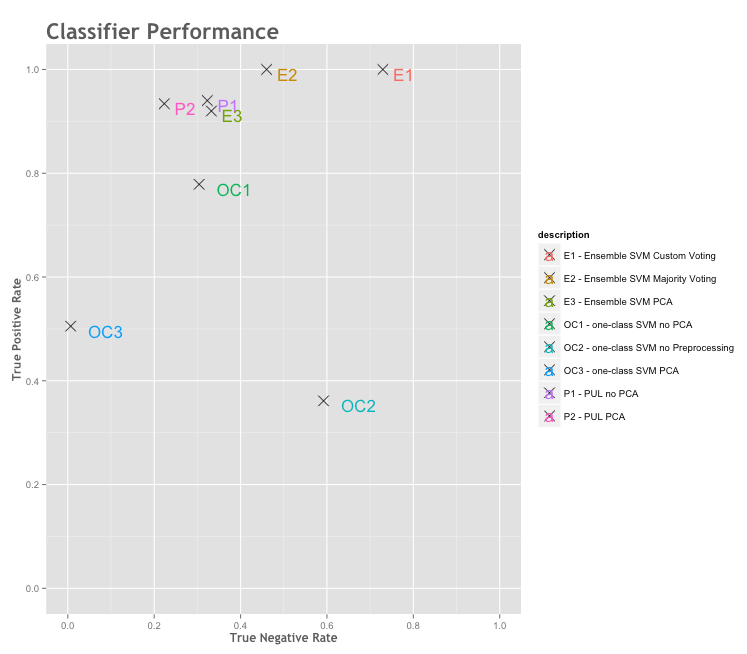
\includegraphics[scale=0.65]{Graphics/classifier-performance.png}
    \caption{An ROC-Graph visualizing the accuracy of the models involved in the experiment.}
    \label{fig:classifier-comparison}
\end{figure}
Again it can be seen that the PUL ensembles were much superior to single algorithms. Except for PCA, all other preprocessing steps enhanced classification performance. Besides it can be seen that the one-class SVM without preprocessing  performance was worse than a random guess without it (see Chapter~\ref{Chapter:4:ROC} for the description how to identify a random classifier by using an ROC Graph). Therefore, it is not surprising that the PUL ensemble without PCA preprocessing is also a winner in this ROC graph, yielding the highest TP and TN rates, which confirms conclusions made from the analysis of the confusion matrices.








 